%!TEX root = ../../thesis.tex

\section{Evaluation}
\label{sec:drqa-eval}

We have all the basic elements of our \sys{DrQA} systems and let's take a look at the evaluation.

\subsection{Question Answering Datasets}
The first question is which question answering datasets we should evaluate on. As we discussed, \sys{SQuAD} is one of the largest general purpose QA datasets currently available for question answering but it is very different from open-domain QA setting. We propose to train and evaluate our system on other datasets developed for open-domain QA that have been constructed in different ways. We hence adopt the following three datasets:

\paragraph{TREC} This dataset is based on the benchmarks from the TREC QA tasks that have been curated by \newcite{baudivs2015modeling}. We use the large version, which contains a total of 2,180 questions extracted from the datasets from TREC 1999, 2000, 2001 and 2002.\footnote{This dataset is available at \url{https://github.com/brmson/dataset-factoid-curated}.} Note that for this dataset, all the answers are written in regular expressions, for example, the answer is \texttt{Sept(ember)?|Feb(ruary)?} to the question \ti{When is Fashion week in NYC?}, so answers \ti{Sept}, \ti{September}, \ti{Feb}, \ti{February} are all judged as correct.

\paragraph{WebQuestions} Introduced in \newcite{berant2013semantic}, this dataset is built to answer questions from the Freebase KB. It was created by crawling questions through the \sys{Google Suggest} API, and then obtaining answers using Amazon Mechanical Turk. We convert each answer to text by using entity names so that the dataset does not reference Freebase IDs and is purely made of plain text question-answer pairs.

\paragraph{WikiMovies} This dataset, introduced in \newcite{miller2016key}, contains 96k question-answer pairs in the domain of movies. Originally created from the \sys{OMDb} and \sys{MovieLens} databases, the examples are built such that they can also be answered by using a subset of Wikipedia as the knowledge source (the title and the first section of articles from the movie domain).

We would like to emphasize that these datasets are not necessarily collected in the context of answering from Wikipedia. The \sys{TREC} dataset was designed for text-based question answering (the primary TREC document sets consist mostly of newswire articles), while \sys{WebQuestions} and \sys{WikiMovies} were mainly collected for knowledge-based question answering. We put all these resources in one unified framework, and test how well our system can answer all the questions --- hoping that it can reflect the performance of general-knowledge QA.

Table~\ref{tab:qa-data-stats} and Figure~\ref{fig:qa-data-stats} give detailed statistics of these QA datasets. As we can see that, the distribution of \sys{SQuAD} examples is quite different from that of the other QA datasets. Due to the construction method, \sys{SQuAD} has longer questions (10.4 tokens vs 6.7--7.5 tokens on average). Also, all these datasets have short answers (although the answers in \sys{SQuAD} are slightly longer) and most of them are factoid.

Note that there are might be multiple answers for many of the questions in these QA datasets (see the \ti{\# answers} column of Table~\ref{tab:qa-data-stats}). For example, there are two valid answers: \ti{English} and \ti{Urdu} to the question \ti{What language do people speak in Pakistan?} on \sys{WebQuestions}. As our system is designed to return one answer, our evaluation considers the prediction as correct if it gives any of the gold answers.

\begin{figure}[h]
\center
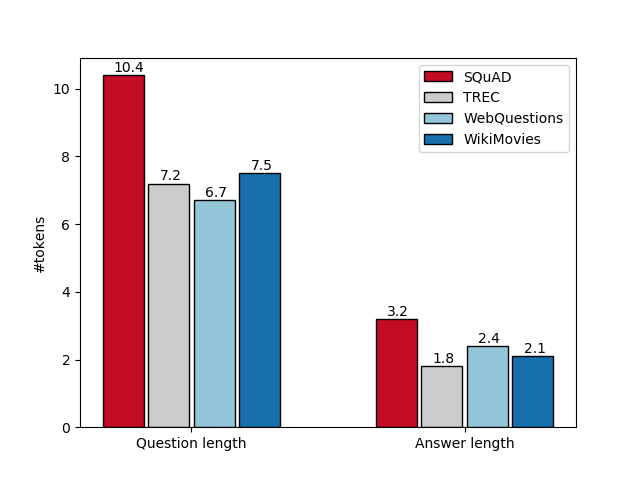
\includegraphics[scale=0.7]{img/qa_stat.png}
\longcaption{The average length of questions and answers in our QA datasets}{\label{fig:qa-data-stats}The average length of questions and answers in our QA datasets. All the statistics are computed based on the training sets.}
\end{figure}

\begin{table}[t]
\begin{center}
\begin{tabular}{l | r r | r | r}
\toprule
\tf{Dataset} & \tf{\# Train} & \tf{\# DS Train} & \tf{\# Test} & \tf{\# answers} \\
\midrule
\sys{SQuAD} & 87,599 & 71,231 & N/A & 1.0  \\
\midrule
\sys{TREC} &  1,486$^{\dagger}$ & 3,464 & 694 & 3.2\footnote{As all the answer strings are regex expressions, it is difficult to estimate \# of answers. We only simply list the number of alternation symbols \texttt{|} in the answer.} \\
\sys{WebQuestions} &  3,778$^{\dagger}$ & 4,602 & 2,032 & 2.4 \\
\sys{WikiMovies} &  96,185$^{\dagger}$ & 36,301 & 9,952 & 1.9 \\
\bottomrule
\end{tabular}
\end{center}
\longcaption{Statistics of the QA datasets used for \sys{DrQA}.}{\label{tab:qa-data-stats} Statistics of the QA datasets used for \sys{DrQA}. DS Train: distantly supervised training data. $^{\dagger}$: These training sets are not used as is because no passage is associated with each question.}
\end{table}




\subsection{Implementation Details}

\subsubsection{Processing Wikipedia}
We use the 2016-12-21 dump\footnote{\url{https://dumps.wikimedia.org/enwiki/latest}} of English Wikipedia for all of our full-scale experiments as the knowledge source used to answer questions. For each page, only the plain text is extracted and all structured data sections such as lists and figures are stripped.\footnote{We use the WikiExtractor script: \url{https://github.com/attardi/wikiextractor}.} After discarding internal disambiguation, list, index, and outline pages, we retain 5,075,182 articles consisting of 9,008,962 unique uncased token types.


\subsubsection{Distantly-supervised data}
We use the following process for each question-answer pair from the training portion of each dataset to build our distantly-supervised training examples. First, we run our \sys{Document Retriever} on the question to retrieve the top 5 Wikipedia articles. All paragraphs from those articles without an exact match of the known answer are directly discarded. All paragraphs  shorter than 25 or longer than 1500  characters are also filtered out. If any named entities are detected in the question, we remove any paragraph that does not contain them at all. For every remaining paragraph in each retrieved page, we score all positions that match an answer using unigram and bigram overlap between the question and a 20 token window, keeping up to the top 5 paragraphs with the highest overlaps. If there is no paragraph with non-zero overlap, the example is discarded; otherwise we add each found pair to our DS training dataset. Some examples are shown in Figure~\ref{fig:ds_examples} and the number of distantly supervised examples we created for training are given in Table~\ref{tab:qa-data-stats} (column \ti{\# DS Train}).


\begin{figure}
\begin{center}
\small
\begin{tabularx}{\textwidth}{l|p{4.5cm}|p{7cm}}
\hline
\bf Dataset & \bf Example & \bf Article / Paragraph \\
\hline
\sys{TREC} & {\bf Q}: What U.S. state's motto is ``Live free or Die''? \newline {\bf A}: New Hampshire & {\bf Article}: Live Free or Die \newline {\bf Paragraph}: ``Live Free or Die'' is the official motto of the U.S. state of \hl{New Hampshire}, adopted by the state in 1945. It is possibly the best-known of all state mottos, partly because it conveys an assertive independence historically found in American political philosophy and partly because of its contrast to the milder sentiments found in other state mottos.\\
\hline
\sys{WebQuestions}  & {\bf Q}: What part of the atom did Chadwick discover?$^\dagger$  \newline {\bf A}: neutron  & {\bf Article}: Atom \newline {\bf Paragraph}: ... The atomic mass of these isotopes varied by integer amounts, called the whole number rule. The explanation for these different isotopes awaited the discovery of the \hl{neutron}, an uncharged particle with a mass similar to the proton, by the physicist James Chadwick in 1932.  ... \\
\hline
\sys{WikiMovies} & {\bf Q}: Who wrote the film Gigli? \newline {\bf A}: Martin Brest &  {\bf Article}: Gigli \newline {\bf Paragraph}: Gigli is a 2003 American romantic comedy film written and directed by \hl{Martin Brest} and starring Ben Affleck, Jennifer Lopez, Justin Bartha, Al Pacino, Christopher Walken, and Lainie Kazan. \\
\hline
\end{tabularx}
\end{center}
\longcaption{Examples of distantly-supervised examples from QA datasets}{\label{fig:ds_examples}Example training data from each QA dataset. In each case we show an associated paragraph where distant supervision (DS) correctly identified the answer within it, which is highlighted.}
\end{figure}


\Subsection{retrieval-eval}{Document Retriever Performance}
We first examine the performance of our retrieval module on all the QA datasets. Table~\ref{tab:ir-res} compares the performance of the two approaches described in Section~\ref{sec:doc-retriever} with that of the Wikipedia Search Engine\footnote{We use the Wikipedia Search API \url{https://www.mediawiki.org/wiki/API:Search}.} for the task of finding articles that contain the answer given a question.

Specifically, we compute the ratio of questions for which the text span of any of their associated answers appear in at least one the top 5 relevant pages returned by each system.

Results on all datasets indicate that our simple approach outperforms Wikipedia Search, especially with bigram hashing. We also compare doing retrieval with Okapi BM25 or by using cosine distance in the word embeddings space (by encoding questions and articles as bag-of-embeddings), both of which we find performed worse.

\begin{table}[t]
\begin{center}
\normalsize
\begin{tabular}{l r r r}
\toprule
\bf Dataset &  \sys{Wiki. Search} & \multicolumn{2}{c}{\sys{Document Retriever}} \\
&    & unigram &  bigram  \\
\midrule
% SQuAD & 62.7 &  76.1 & \bf 77.8 \\
% %\curq  & 82.8 & 84.2 & \bf 85.6 \\
\sys{TREC} & 81.0 & 85.2 & \bf 86.0 \\
\sys{WebQuestions} &    73.7 & \bf 75.5 & 74.4 \\
\sys{WikiMovies} & 61.7 &  54.4 &  \bf 70.3 \\
\bottomrule
\end{tabular}
\end{center}
\longcaption{Document retrieval results}{\label{tab:ir-res} Document retrieval results. \% of questions for which the answer segment appears in one of the top 5 pages returned by the method. }
\end{table}


\subsection{Final Results}
\label{sec:drqa-final-results}
Finally, we assess the performance of our full system \sys{DrQA} for answering open-domain questions using all these datasets. We compare three versions of \sys{DrQA} which evaluate the impact of using distant supervision and multitask learning across the training sources provided to \sys{Document Reader} (\sys{Document Retriever} remains the same for each case):

\begin{itemize}
\item
  \sys{SQuAD}: A single \sys{Document Reader} model is trained on the \sys{SQuAD} training set only and used on all evaluation sets. We used the model that we described in Section~\ref{sec:drqa} (the F1 score is 79.0\% on the test set of \sys{SQuAD}).
\item
  Fine-tune (DS): A \sys{Document Reader} model is pre-trained on \sys{SQuAD} and then fine-tuned for each dataset independently using its distant supervision (DS) training set.
\item
  Multitask (DS): A single \sys{Document Reader} model is jointly trained on the SQuAD training set and all the distantly-supervised examples.
\end{itemize}

For the full Wikipedia setting we use a streamlined model that does not use the \sys{CoreNLP} parsed $f_{token}$ features or lemmas for $f_{exact\_match}$. We find that while these help for more exact paragraph reading in \sys{SQuAD}, they don't improve results in the full setting. Additionally, \sys{WebQuestions} and \sys{WikiMovies} provide a list of candidate answers (1.6 million \sys{Freebase} entity strings for \sys{WebQuestions} and 76k movie-related entities for \sys{WikiMovies}) and we restrict that the answer span must be in these lists during prediction.

Table~\ref{tab:drqa-full-results} presents the results. We only consider top-1, exact-match accuracy, which is the most restricted and challenging setting. In the original paper \cite{chen2017reading}, we also evaluated the question/answer pairs in SQuAD. We omit them here because that at least a third of these questions are context-dependent and are not really suitable for open QA.

\begin{table}[t]
\begin{center}
\begin{tabular}{l c ccc cc}
\toprule
\textbf{Dataset} &  \tf{YodaQA} &  \multicolumn{3}{c}{\tf{DrQA}} & \multicolumn{2}{c}{\tf{DrQA*}} \\
&   &  {SQuAD} &  {FT} & {MT} & {SQuAD} & {FT} \\
\midrule
\sys{TREC} & 31.3 & 19.7 & 25.7 & 25.4 &  21.3 &  28.8 \\
\sys{WebQuestions} & 38.9 & 11.8 & 19.5 & 20.7 & 14.2 & 24.3 \\
\sys{WikiMovies} & N/A & 24.5 & 34.3 & 36.5 & 31.9 & 46.0 \\
\bottomrule
\end{tabular}
\end{center}
\longcaption{Final performance of DrQA}{\label{tab:drqa-full-results} Full Wikipedia results. Top-1 exact-match accuracy (\%). \tf{FT}: Fine-tune (DS). \tf{MT}: Multitask (DS). The \sys{DrQA*} results are taken from \newcite{raison2018weaver}.}
\end{table}

Despite the difficulty of the task compared to the reading comprehension task (where you are given the right paragraph) and unconstrained QA (using redundant resources), \sys{DrQA} still provides reasonable performance across all four datasets.

We are interested in a single, full system that can answer any question using Wikipedia. The single model trained only on \sys{SQuAD} is outperformed on all the datasets by the multitask model that uses distant supervision. However, performance when training on SQuAD alone is not far behind, indicating that task transfer is occurring. The majority of the improvement from \sys{SQuAD} to Multitask (DS) learning, however, is likely not from task transfer, as fine-tuning on each dataset alone using DS also gives improvements, showing that is the introduction of extra data in the same domain that helps. Nevertheless, the best single model that we can find is our overall goal, and that is the Multitask (DS) system.

We compare our system to \sys{YodaQA} \cite{baudivs2015yodaqa} (an unconstrained QA system using redundant resources), giving results which were previously reported on \sys{TREC} and \sys{WebQuestions}.\footnote{The results are extracted from \href{https://github.com/brmson/yodaqa/wiki/Benchmarks}{https://github.com/brmson/yodaqa/wiki/Benchmarks}.} Despite the increased difficulty of our task, it is reassuring that our performance is not too far behind on \sys{TREC} (31.3 vs 25.4). The gap is slightly bigger on \sys{WebQuestions}, likely because this dataset was created from the specific structure of \sys{Freebase} which \sys{YodaQA} uses directly.

We also include the results from an enhancement of our model named \sys{DrQA*}, presented in \newcite{raison2018weaver}. The biggest change is that this reading comprehension model is trained and evaluated directly on the Wikipedia articles instead of paragraphs (documents are on average 40 times larger than individual paragraphs). As we can see, the performance has been improved consistently on all the datasets, and the gap from \sys{YodaQA} is hence further reduced.

\clearpage
\begin{longtable}{l l p{12cm}}
\hline
(a) & \tf{Question} & What is question answering? \\
& \tf{Answer} & a computer science discipline within the fields of information retrieval and natural language processing \\
& \tf{Wiki. article} & \href{https://en.wikipedia.org/wiki/Question_answering}{Question Answering} \\
& \tf{Passage} & {\small Question Answering (QA) is \hl{a computer science discipline within the fields of information retrieval and natural language processing} (NLP), which is concerned with building systems that automatically answer questions posed by humans in a natural language.} \\
\hline
(b) & \tf{Question} & Which state is Stanford University located in? \\
& \tf{Answer} & California \\
& \tf{Wiki. article} & \href{https://en.wikipedia.org/wiki/Stanford_Memorial_Church}{Stanford Memorial Church} \\
& \tf{Passage} & {\small Stanford Memorial Church (also referred to informally as MemChu) is located on the Main Quad at the center of the Stanford University campus in Stanford, \hl{California}, United States. It was built during the American Renaissance by Jane Stanford as a memorial to her husband Leland. Designed by architect Charles A. Coolidge, a protégé of Henry Hobson Richardson, the church has been called "the University's architectural crown jewel".} \\
\hline
(c) & \tf{Question} & Who invented LSTM? \\
& \tf{Answer} & Sepp Hochreiter \& J\"urgen Schmidhuber \\
& \tf{Wiki. article}  & \href{https://en.wikipedia.org/wiki/Deep_learning}{Deep Learning} \\
& \tf{Passage} & {\small Today, however, many aspects of speech recognition have been taken over by a deep learning method called Long short-term memory (LSTM), a recurrent neural network published by \hl{Sepp Hochreiter \& J\"urgen Schmidhuber} in 1997. LSTM RNNs avoid the vanishing gradient problem and can learn ``Very Deep Learning'' tasks that require memories of events that happened thousands of discrete time steps ago, which is important for speech. In 2003, LSTM started} \\
& & {\small  to become competitive with traditional speech recognizers on certain tasks. Later it was combined with CTC in stacks of LSTM RNNs. In 2015, Google's speech recognition reportedly experienced a dramatic performance jump of 49\% through CTC-trained LSTM, which is now available through Google Voice to all smartphone users, and has become a show case of deep learning.} \\
\hline
(d) & \tf{Question} & What is the answer to life, the universe, and everything? \\
& \tf{Answer} & 42 \\
& \tf{Wiki. article} & \href{https://en.wikipedia.org/wiki/Phrases_from_The_Hitchhiker%27s_Guide_to_the_Galaxy}{Phrases from The Hitchhiker's Guide to the Galaxy} \\
& \tf{Passage} & {\small The number 42 and the phrase, "Life, the universe, and everything" have attained cult status on the Internet. "Life, the universe, and everything" is a common name for the off-topic section of an Internet forum and the phrase is invoked in similar ways to mean "anything at all". Many chatbots, when asked about the meaning of life, will answer "42". Several online calculators are also programmed with the Question. Google Calculator will give the result to "the answer to life the universe and everything" as 42, as will Wolfram's Computational Knowledge Engine. Similarly, DuckDuckGo also gives the result of "the answer to the ultimate question of life, the universe and everything" as \hl{42}. In the online community Second Life, there is a section on a sim called "42nd Life." It is devoted to this concept in the book series, and several attempts at recreating Milliways, the Restaurant at the End of the Universe, were made.} \\
\hline
\longcaption{Sample predictions of our \sys{DrQA} system}{\label{tab:drqa-output}Sample predictions of our \sys{DrQA} system.}
\end{longtable}

Lastly, our \sys{DrQA} system is open-sourced at \href{https://github.com/facebookresearch/DrQA}{https://github.com/facebookresearch/DrQA} (the Multitask (DS) system was deployed). Table~\ref{tab:drqa-output} lists some sample predictions that we tried by ourselves (not in any of these datasets). As is seen, our system is able to return a precise answer to all these factoid questions and answering some of these questions is not trivial:

\begin{enumerate}[(a)]
    \item It is not trivial to identify that \ti{a computer science discipline within the fields of information retrieval and natural language processing} is the complete noun phrase and the correct answer although the question is pretty simple.
    \item Our system finds the answer in another Wikipedia article \ti{Stanford Memorial Church}, and gives the exactly correct answer \ti{California} as the \ti{state} (instead of \ti{Stanford} or \ti{United States}).
    \item To get the correct answer, the system needs to understand the syntactic structure of the question and the context \ti{Who invented LSTM?} and \ti{a deep learning method called Long short-term memory (LSTM), a recurrent neural network published by Sepp Hochreiter \& J\"urgen Schmidhuber in 1997.}
\end{enumerate}

Conceptually, our system is simple and elegant, and doesn't rely on any additional linguistic analysis or external or hand-coded resources (e.g., dictionaries). We think this approach holds great promise for a new generation of open-domain question answering systems. In the next section, we discuss current limitations and possible directions for further improvement.
